\section{How the Position of the Sun, the Moon, and the Ascendant at the Conception Can Be Accurately Found (13K,10P)}

We will explain an economical method for finding the latitude. 

For every nativity, the sign square with the \Sun\xspace is the sign of the conception. (Occasionally the sign of conception will be trine when the \Sun\xspace happens to be at the end of its sign, especially in a sign of short rising time; the sign of conception may be sextile for signs of long rising time.) 

Assume the position of the \Moon\xspace at the conception to be the same as the position of the Ascendant at the time of the delivery, and from this you can know whether the conception was at new or full moon.

An example: \Sun\xspace in \Aquarius, \Moon\xspace in \Scorpio, Ascendant in \Virgo. At the conception the \Sun\xspace was
in \Taurus, the \Moon\xspace in \Virgo. It is clear that the conception was at new moon, for the \Moon\xspace (i.e. the
Ascendant) had not yet come into opposition to the position of the \Sun\xspace at the conception. 

If the Ascendant at the delivery is found to be past its opposition to the \Sun\xspace at conception, the conception will be at full moon.

It is necessary to establish the vital sectors for the conception in the same way as was explained for the delivery. In most cases a native whose conception was at new moon \textbf{/145P/} will die at full moon; one whose conception was at full moon will die at new moon.

\textbf{/153K/} Another <topic>: having determined in which sign the <preceding> new or full \Moon\xspace occurred, count the degrees from that point in the order of the signs to the ascending node. Then count the total distance from the Ascendant “downwards” (=in the order of signs) for day births, in the direction of diurnal motion (=towards MC) for night births. 

If, however, the ascending node is at MC, it is necessary to count the distance in degrees from MC, in the order of the signs towards the Ascendant for day births, in the direction of diurnal motion towards the Descendant for night births. 

If the ascending node is at the Descendant, count the distance from the Descendant to MC for day births, to IC for night births. 

If the ascending node happens to be at IC, then count the distance in degrees in the direction of diurnal motion
from IC towards the Ascendant, if the birth is found to be during the day; for night births count toward the Descendant from IC. 

\enlargethispage{2\baselineskip}
\clearpage
\begin{wrapfigure}[16]{R}{7cm}
\centering
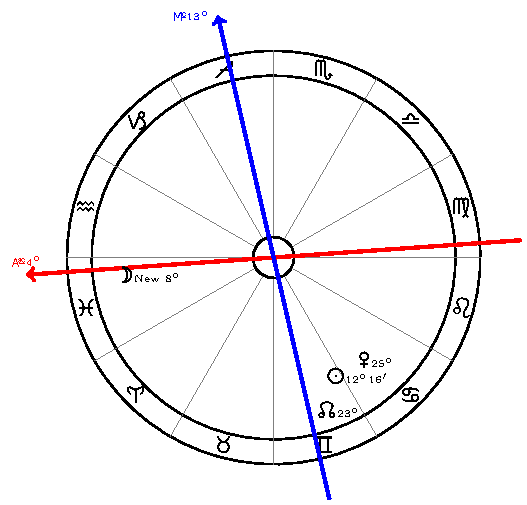
\includegraphics[width=0.68\textwidth]{charts/3_13_1}
\caption{Chart 46 [III.13.1, GH L75,I]}
\label{fig:chart46}
\end{wrapfigure}

For example: the ascending node at \Gemini\xspace 23°, the <preceding> new moon at \Pisces\xspace 8°, the Ascendant at \Pisces\xspace 4°, MC at \Sagittarius\xspace 13°
\footnote{\textit{Greek Horoscopes} gives the chart as L75,I to but can't date it accurately due to discrepancies (p.89)}. 

I take the distance from the new moon to the ascending node; this is 105°. I count this from the Ascendant (since it was a day birth) and stop at \Gemini\xspace 19°. For the second klima the total is approximately 79 years, <4> months\footnote{Robert Hand calculates this using ascenion times of \Pisces\, 20°, \Aries\, 20°, \Taurus\, 24°, and \Gemini\, 28°. Which gives (26/30 x 20) + 20 + 24 + (19/30 x 28) = 17.33 + 44 + 17.73 = 79.06 $\approx$ 79 years 1 month (VRS3 p65)}. The native lived that long.

I have explained the systems which I myself have used. I have investigated nativities, observing if two, three, or more of the previously mentioned factors coincide, yielding the same result, and through this investigation I have made infallible forecasts of deaths. As a result it is not without plan, not at random, that I have explained that each method is quite practicable both by itself and when combined with another. If anyone sticks to these methods, he will find a true forecast of the subjects in question to be within his grasp. 

\hl{Now we have written some parts of our work mystically, leaving something to the discrimination and the judgement of our readers\footnote{Valens is telling us his text needs close reading if we are to get full value from it.}.} In doing so we have not been led by malice or stupidity, but by our wish to supply the student with point of interest and opportunities for long discussion. For <we know> that if anyone attains his longed-for goals without being challenged, he considers it a trivial gift, but one
who attains them after a toilsome search engages in his activity not only with pleasure but with success.

\newpage
\clearpage
\begin{wrapfigure}[13]{R}{7cm}
\centering
\vspace{-20pt}
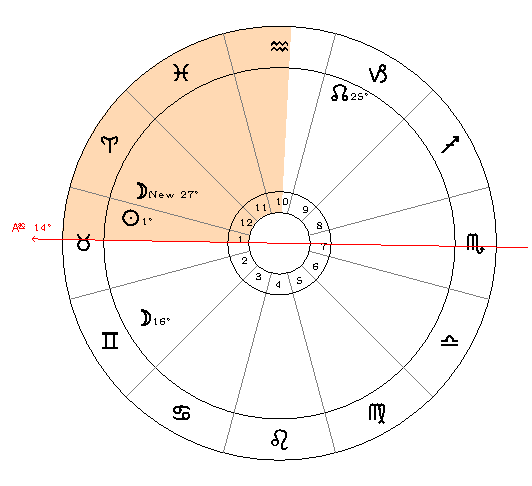
\includegraphics[width=0.68\textwidth]{charts/3_13_2}
\caption{Chart 47 [III.13.2, GH L74,IV]}
\label{fig:chart47}
\end{wrapfigure}

\noindent \textbf{/154K;146P/} An example: \Sun\xspace in \Taurus\xspace 1°, \Moon\xspace in \Gemini\xspace 16°, Ascendant in \Taurus\xspace 14°, the <previous> new moon in \Aries\xspace 27°, the ascending node in \Capricorn\xspace 25°\footnote{\textit{Greek Horoscopes} dates the chart (L74,IV) to approximately April 19, 74 AD (p.86)}.

I counted in the direction of diurnal motion from the position of the new moon to the ascending node; the distance is 92°. 

I counted this distance in the direction of diurnal motion from the degree-position of the Ascendant and came to \Aquarius\xspace 12°. 

The 92° total for the klima of Alexandria equals 70 years\footnote{Robert Hand does not give a calculation for this. Going in diurnal motion, the Ascendant would have to rise thru the first 14° of \Taurus, all of \Aries\, and \Pisces, and the last 18° of \Aquarius. The ascenional times of these signs are: \Taurus\, 24°,  \Aries\, and \Pisces\, 20° each, and \Aquarius, 24° so the calculation is: (14/30 x 24) + 20 + 20 + (18/30 x 24) = 11.2 + 40 + 14.4 = 68.4 $\approx$ 68 years 5 months; not quite the 70 years Valens arrived at.}. The native died in the first month of his seventieth year. 

The method according to the conception is as follows: since the full moon <preceding> the conception was at \Capricorn\xspace 21° \ldots which is close to the year we found previously.

\newpage
Another example: \Sun\xspace in \Aquarius\xspace 29°, \Moon\xspace in the beginning of \Aries, Ascendant in \Capricorn\xspace 18°,
the <preceding> n[e]w moon in \Aquarius\xspace 26°, the ascending node in \Scorpio\xspace 16°
\footnote{\textit{Greek Horoscopes} dates the chart (L115,II) to approximately February 15, 115 AD (p.112)}.

\clearpage
\begin{wrapfigure}[14]{R}{7cm}
\centering
\vspace{-20pt}
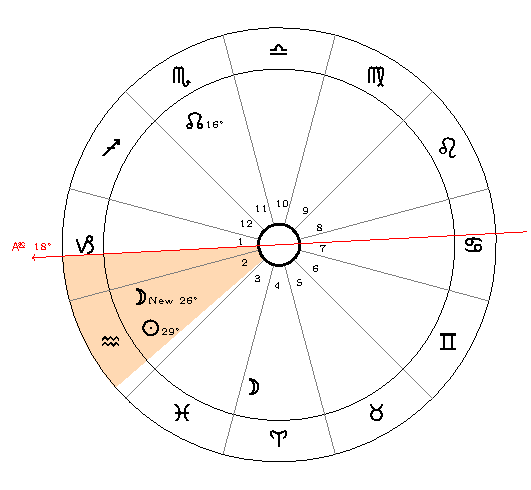
\includegraphics[width=0.68\textwidth]{charts/3_13_3}
\caption{Chart 48 [III.13.3, GH L115,II]}
\label{fig:chart48}
\end{wrapfigure}

I counted the distance from the new moon in the direction of diurnal motion to the degree-position of the Ascendant; the distance is 38°. I counted this in the order of the signs\footnote{He is treating this as a diurnal chart even though the \Sun\, is below the horizon probably because the \Moon\, is in the 4th an the \Sun\, will rise ahead of it.} from the degree-position of the Ascendant. The years total very nearly 33 in the first klima. He lived 32 years 5 months\footnote{Robert Hand computes this using ascension times of \Capricorn\, as 28° and those of \Aquarius\, as 24° giving: (12/30 x 28) + (26/30 x 24) = 11.2 + 20.8 = 32 years (VRS3 p66).}. 

The place of the conception did not contain the apheta because the full moon of the conception and the ascending node happened to be at the same degree-position. Therefore he had a dangerous birth and a violent end.

\newpage